% ==============================================================================
% ENTREGA 2 -- ARTIGO CIENTÍFICO (PADRÃO ESTRITO ABNT, MÁX. 10 PÁGINAS)
% Teoria do Aprendizado Estatístico -- Tecnologia em Ciência de Dados
% Fatec Baixada Santista -- Rubens Lara | Grupo APPA
% Normas aplicadas: NBR 6022:2018, NBR 10520:2023, NBR 6023:2018,
%                   NBR 6028:2021, NBR 6024:2012, NBR 14724 e IBGE (1993).
% Compile na raiz do repositório com: Rscript entregas/entrega-2/compilar-entrega-2.R
% ==============================================================================

\documentclass[
  article,
  12pt,
  oneside,
  a4paper,
  section=TITLE,
  english,
  brazil
]{abntex2}\usepackage[]{graphicx}\usepackage[]{xcolor}
% maxwidth is the original width if it is less than linewidth
% otherwise use linewidth (to make sure the graphics do not exceed the margin)
\makeatletter
\def\maxwidth{ %
  \ifdim\Gin@nat@width>\linewidth
    \linewidth
  \else
    \Gin@nat@width
  \fi
}
\makeatother

\definecolor{fgcolor}{rgb}{0.345, 0.345, 0.345}
\newcommand{\hlnum}[1]{\textcolor[rgb]{0.686,0.059,0.569}{#1}}%
\newcommand{\hlsng}[1]{\textcolor[rgb]{0.192,0.494,0.8}{#1}}%
\newcommand{\hlcom}[1]{\textcolor[rgb]{0.678,0.584,0.686}{\textit{#1}}}%
\newcommand{\hlopt}[1]{\textcolor[rgb]{0,0,0}{#1}}%
\newcommand{\hldef}[1]{\textcolor[rgb]{0.345,0.345,0.345}{#1}}%
\newcommand{\hlkwa}[1]{\textcolor[rgb]{0.161,0.373,0.58}{\textbf{#1}}}%
\newcommand{\hlkwb}[1]{\textcolor[rgb]{0.69,0.353,0.396}{#1}}%
\newcommand{\hlkwc}[1]{\textcolor[rgb]{0.333,0.667,0.333}{#1}}%
\newcommand{\hlkwd}[1]{\textcolor[rgb]{0.737,0.353,0.396}{\textbf{#1}}}%
\let\hlipl\hlkwb

\usepackage{framed}
\makeatletter
\newenvironment{kframe}{%
 \def\at@end@of@kframe{}%
 \ifinner\ifhmode%
  \def\at@end@of@kframe{\end{minipage}}%
  \begin{minipage}{\columnwidth}%
 \fi\fi%
 \def\FrameCommand##1{\hskip\@totalleftmargin \hskip-\fboxsep
 \colorbox{shadecolor}{##1}\hskip-\fboxsep
     % There is no \\@totalrightmargin, so:
     \hskip-\linewidth \hskip-\@totalleftmargin \hskip\columnwidth}%
 \MakeFramed {\advance\hsize-\width
   \@totalleftmargin\z@ \linewidth\hsize
   \@setminipage}}%
 {\par\unskip\endMakeFramed%
 \at@end@of@kframe}
\makeatother

\definecolor{shadecolor}{rgb}{.97, .97, .97}
\definecolor{messagecolor}{rgb}{0, 0, 0}
\definecolor{warningcolor}{rgb}{1, 0, 1}
\definecolor{errorcolor}{rgb}{1, 0, 0}
\newenvironment{knitrout}{}{} % an empty environment to be redefined in TeX

\usepackage{amsmath}
\usepackage{alltt}

% --- Codificação, idioma e tipografia ABNT (Times, 12pt) ---
\usepackage[T1]{fontenc}
\usepackage[utf8]{inputenc}
\usepackage[nott]{newtxtext}
\usepackage{newtxmath}
\renewcommand{\ttdefault}{lmtt}
\usepackage[expansion=false]{microtype}
\usepackage{indentfirst}
\usepackage{csquotes}

% --- Matemática, tabelas IBGE e gráficos ---
\usepackage{amsmath}
\usepackage{icomma}
\usepackage{booktabs}
\usepackage{array}
\usepackage{graphicx}
\usepackage{xurl}

% --- Legendas ABNT / IBGE (fonte reduzida, alinhamento à esquerda, recuo pendente) ---
\hangcaption
\captionstyle{\raggedright}
\captionnamefont{\ABNTEXfontereduzida}
\captiontitlefont{\ABNTEXfontereduzida}

% --- Espaçamento e margens estritas ABNT: 3 cm (sup/esq) e 2 cm (inf/dir) ---
\OnehalfSpacing
\setlrmarginsandblock{3cm}{2cm}{*}
\setulmarginsandblock{3cm}{2cm}{*}
\setheadfoot{14.5pt}{14pt}
\setheaderspaces{*}{0.65cm}{*}
\checkandfixthelayout[fixed]
\setlength{\parindent}{1.25cm}
\setlength{\parskip}{0pt}
\clubpenalty=10000
\widowpenalty=10000
\displaywidowpenalty=10000
\setbeforesecskip{10pt}
\setaftersecskip{5pt}
\setbeforesubsecskip{7pt}
\setaftersubsecskip{3.5pt}
\setlength{\intextsep}{7pt plus 2pt minus 2pt}
\setlength{\textfloatsep}{8pt plus 2pt minus 2pt}
\setlength{\floatsep}{7pt plus 2pt minus 2pt}

% --- Hierarquia tipográfica dos títulos (NBR 6024:2012, fonte 12pt uniforme) ---
\renewcommand{\ABNTEXchapterfont}{\normalfont\bfseries}
\renewcommand{\ABNTEXsectionfont}{\normalfont\bfseries}
\renewcommand{\ABNTEXsectionfontsize}{\normalsize}
\renewcommand{\ABNTEXsubsectionfont}{\normalfont\bfseries}
\renewcommand{\ABNTEXsubsectionfontsize}{\normalsize}
\renewcommand{\ABNTEXsubsubsectionfont}{\normalfont\itshape}
\renewcommand{\ABNTEXsubsubsectionfontsize}{\normalsize}
\setsecheadstyle{\ABNTEXsectionfont\ABNTEXsectionfontsize\ABNTEXsectionupperifneeded}
\setsubsecheadstyle{\ABNTEXsubsectionfont\ABNTEXsubsectionfontsize}
\setsubsubsecheadstyle{\ABNTEXsubsubsectionfont\ABNTEXsubsubsectionfontsize}

% --- Bibliografia e citações estritas NBR 10520:2023 e NBR 6023:2018 ---
\usepackage[
  backend=biber,
  style=abnt,
  giveninits=false,
  repeatfields,
  maxcitenames=3,
  mincitenames=1,
  maxbibnames=3,
  minbibnames=1,
  uniquename=false,
  uniquelist=false
]{biblatex}
\addbibresource{referencias.bib}

% Força entrada de referências alinhada à esquerda, espaço simples e separação limpa
\AtBeginBibliography{%
  \SingleSpacing
  \raggedright
  \setlength{\bibitemsep}{0.65\baselineskip}
}

% --- Hiperlinks e metadados PDF ---
\hypersetup{
  hidelinks,
  pdftitle={Sinistros de trânsito em horários de pico no Estado de São Paulo: acurácia, sensibilidade e interpretação na regressão logística},
  pdfauthor={Arthur Galvão; Pedro Henrique; Ailana Pereira Gonsalez},
  pdflang={pt-BR}
}

\titulo{SINISTROS DE TRÂNSITO EM HORÁRIOS DE PICO NO ESTADO DE SÃO PAULO: ACURÁCIA, SENSIBILIDADE E INTERPRETAÇÃO NA REGRESSÃO LOGÍSTICA}
\tituloestrangeiro{Traffic Crashes during Peak Hours in the State of São Paulo: Accuracy, Sensitivity, and Interpretation in Logistic Regression}
\autor{Grupo APPA}
\local{Santos-SP}
\data{27 de novembro de 2026}
\IfFileExists{upquote.sty}{\usepackage{upquote}}{}
\begin{document}



\selectlanguage{brazil}
\frenchspacing
\pagestyle{abntchapfirst}
\thispagestyle{abntchapfirst}

% ==============================================================================
% ELEMENTOS PRÉ-TEXTUAIS (ABNT NBR 6022:2018 e NBR 6028:2021)
% ==============================================================================
\begin{SingleSpace}
\begin{center}
  {\normalsize\bfseries\imprimirtitulo\par}
  \vspace{0.18em}
  {\normalsize\itshape\imprimirtituloestrangeiro\par}
  \vspace{0.3em}
  {\normalsize
    Arthur Galvão\footnotemark[1] \quad
    Pedro Henrique\footnotemark[1] \quad
    Ailana Pereira Gonsalez\footnotemark[1]\par}
  \vspace{0.18em}
  {\footnotesize
    Fatec Baixada Santista -- Rubens Lara, Santos-SP \quad|\quad Ciência de Dados \quad|\quad Grupo: APPA \\
    Teoria do Aprendizado Estatístico \quad|\quad Prof.\ Dr.\ João Paulo Ferreira de Mello \quad|\quad 27 nov.\ 2026%
  \par}
\end{center}
\end{SingleSpace}

\footnotetext[1]{Discentes do Curso Superior de Tecnologia em Ciência de Dados, Fatec Baixada Santista -- Rubens Lara, Santos-SP.}

\vspace{0.15em}

\begin{SingleSpace}
\noindent\makebox[\linewidth]{\textbf{RESUMO}}

\vspace{0.12em}
\noindent Este estudo investiga características registradas associadas a sinistros de trânsito em horários de pico no Estado de São Paulo a partir de 151.175 boletins policiais válidos do Infosiga-SP (janeiro de 2025 a junho de 2026), após exclusão de notificações e de 658 registros incompletos (656 fatais). O alvo binário \texttt{pico} (06h30--08h30, 11h30--13h30 e 17h00--19h30) é modelado por tipo de via, dia da semana e região administrativa via regressão logística ajustada em 2025 ($n = 101.666$) e avaliada no primeiro semestre de 2026 ($n = 49.509$). No teste temporal, o modelo obtém 59,43\% de acurácia (29.424 acertos, quatro acima da referência constante de 59,42\%), Brier de 0,237184 ($\mathrm{RMSE} = 0{,}487015$) e AUC de 0,5757, mas identifica apenas 371 dos 20.089 casos de pico em $\tau = 0{,}5$ (1,85\% de sensibilidade), sem implicar inferência causal.\par

\vspace{0.12em}
\noindent\textbf{Palavras-chave:} regressão logística; sinistros de trânsito; horários de pico; validação temporal; Infosiga-SP.
\end{SingleSpace}

\vspace{0.25em}

\begin{SingleSpace}
\begin{otherlanguage}{english}
\noindent\makebox[\linewidth]{\textbf{ABSTRACT}}

\vspace{0.12em}
\noindent This study investigates recorded crash attributes associated with peak hours in the State of São Paulo using 151,175 valid police reports from Infosiga-SP (January 2025 to June 2026), after excluding notifications and 658 incomplete records (656 fatal). The binary \texttt{pico} target (06:30--08:30, 11:30--13:30, and 17:00--19:30) is modeled exclusively by road type, day of the week, and administrative region via logistic regression fitted on 2025 ($n = 101,666$) and evaluated on the first half of 2026 ($n = 49,509$). On the temporal test set, the model achieves 59.43\% accuracy (29,424 correct predictions, four above the 59.42\% constant baseline), Brier score 0.237184 ($\mathrm{RMSE} = 0.487015$), and AUC 0.5757, yet identifies only 371 of 20,089 peak cases at $\tau = 0.5$ (1.85\% sensitivity), without causal inference.\par

\vspace{0.12em}
\noindent\textbf{Keywords:} logistic regression; traffic crashes; peak hours; temporal validation; Infosiga-SP.
\end{otherlanguage}
\end{SingleSpace}

\textual
\pagestyle{abntchapfirst}
\OnehalfSpacing

% ==============================================================================
\section{Introdução}
% ==============================================================================

A segurança viária constitui eixo estratégico de saúde pública e gestão da mobilidade urbana, requerendo análises quantitativas transparentes sobre registros padronizados de ``sinistros de trânsito'', expressão normativa adotada em substituição a ``acidente'' por enfatizar o caráter evitável dos eventos \parencite{who2010,abnt10697}. Embora a concentração de ocorrências em horários de deslocamento pendular seja associada ao aumento do tráfego, bases administrativas registram apenas eventos ocorridos, omitindo o volume de viagens incólumes e impossibilitando estimar risco causal por veículo em circulação \parencite{who2010}. Diante dessa restrição observacional e dos princípios do aprendizado estatístico voltado à inferência descritiva \parencite{james2021}, investiga-se nos dados do Infosiga-SP \parencite{infosiga2026}: \textbf{que características registradas dos sinistros de trânsito estão associadas ao pertencimento aos horários de pico?}

Para operacionalizar a resposta sem vazamento de informação, o alvo binário \texttt{pico} classifica cada boletim policial conforme três janelas diárias (06h30--08h30, 11h30--13h30 e 17h00--19h30), empregando apenas tipo de via, dia da semana e região administrativa em regressão logística ajustada em 2025 e avaliada no primeiro semestre de 2026 --- mantendo hora e turno fora das preditoras por determinarem mecanicamente o próprio alvo. No teste temporal, o modelo obtém 59,43\% de acurácia global (29.424 acertos em 49.509 boletins), apenas quatro acertos acima da referência constante, enquanto identifica somente 371 dos 20.089 boletins no pico (sensibilidade de 1,85\%). Assim, o artigo formaliza a preparação e auditoria dos dados, estima as razões de chances condicionadas, decompõe métricas probabilísticas e categóricas e explicita os limites metodológicos do ajuste.

% ==============================================================================
\section{Fundamentação teórica}
% ==============================================================================

No aprendizado estatístico, relaciona-se a resposta $Y$ aos preditores $X = (X_1, \ldots, X_p)$ por $Y = f(X) + \varepsilon$, atendendo aos objetivos de \textit{predição} fora da amostra e \textit{inferência} sobre a magnitude e o sinal das associações \parencite{james2021,hastie2009}. Para resposta binária $Y \in \{0, 1\}$, a regressão logística especifica a ligação canônica logito nos Modelos Lineares Generalizados \parencite{mccullagh1989,james2021}:
\begin{equation}
  \eta(x) = \log\!\left(\frac{p(x)}{1 - p(x)}\right) = \beta_0 + \sum_{j=1}^{p} \beta_j x_j,
  \qquad
  p(x) = \frac{1}{1 + e^{-\eta(x)}},
\end{equation}
com estimação por máxima verossimilhança e razões de chances ajustadas $\mathrm{OR}_j = \exp(\beta_j)$ na escala de \textit{odds} \parencite{bruce2019}.

Em séries cronológicas, a validação temporal evita avaliar sobre o mesmo conjunto do ajuste \parencite{hastie2009}, mas a reutilização prévia do período de teste caracteriza validação retrospectiva, demandando documentação transparente de filtragens, variáveis excluídas, partições e referência \parencite{lones2024,kapoor2024}. Antes da escolha de corte, regras estritamente próprias como o escore de Brier $\mathrm{Brier} = n^{-1}\sum_{i=1}^{n}(y_i - \hat{p}_i)^2$ \parencite{brier1950}, sua raiz $\mathrm{RMSE} = \sqrt{\mathrm{Brier}}$ e o log-loss medem erro probabilístico, enquanto a Área sob a Curva ROC (AUC) resume a ordenação entre positivos e negativos (valendo $0{,}5$ ao acaso e $1{,}0$ na separação perfeita) \parencite{james2021,bruce2019}. Sob limiar fixo $\tau$ (usualmente $\tau = 0{,}5$), a matriz de confusão gera métricas com numeradores e denominadores distintos:
{\small
\begin{equation}
  \text{Acurácia} = \frac{\mathrm{VP} + \mathrm{VN}}{\mathrm{VP} + \mathrm{VN} + \mathrm{FP} + \mathrm{FN}}, \quad
  \mathrm{Sensibilidade} = \frac{\mathrm{VP}}{\mathrm{VP} + \mathrm{FN}}, \quad
  \mathrm{Especificidade} = \frac{\mathrm{VN}}{\mathrm{VN} + \mathrm{FP}},
\end{equation}
}
nas quais probabilidades concentradas abaixo de $0{,}5$ podem produzir acurácia próxima à da classe majoritária acompanhada de baixa sensibilidade \parencite{bruce2019,lones2024}. A calibração conjunta das previsões é verificada por regressão logística do desfecho sobre $\operatorname{logit}(\hat{p}_i)$ (hipótese nula de intercepto $0$ e inclinação $1$).

Em registros diários de trânsito, fatores climáticos e sazonais induzem dependência intradiária que invalida erros-padrão convencionais; por isso empregam-se covariâncias sanduíche robustas agrupadas por data (\textit{cluster-robust} HC1) \parencite{zeileis2020}, testes conjuntos de Wald $W = \hat{\boldsymbol{\beta}}_S^{\mathsf{T}} \hat{\mathbf{V}}_{S,\mathrm{CL}}^{-1} \hat{\boldsymbol{\beta}}_S \sim \chi^2_g$ com correção sequencial de \textcite{holm1979} para controle da taxa de erro familiar (FWER) e bootstrap circular em blocos de sete dias para estimar a incerteza temporal do contraste de Brier \parencite{politis1992,efron1993}.

% ==============================================================================
\section{Materiais e métodos}
% ==============================================================================

Os dados provêm do registro aberto oficial do Infosiga-SP, mantido pelo \textcite{infosiga2026}, em cópia versionada localmente com 273.371 registros e 50 variáveis (1º jan.\ 2025 a 30 jun.\ 2026; 546 dias; 645 municípios; 16 regiões). Na leitura em \textit{Latin-1} com aspas respeitadas, corrigiu-se desalinhamento anterior de leitura (que gerava 273.372 linhas) e filtraram-se apenas os 151.833 boletins policiais únicos de sinistros fatais e não fatais, removendo as 121.538 notificações administrativas (estrutura distinta), sem duplicidades e com dia da semana 100\% compatível com o calendário. Excluíram-se 242 boletins sem data/horário válidos e, dentre os 151.591 restantes, 416 sem tipo de via informado, resultando em 151.175 boletins completos (sem perdas adicionais nas preditoras), conforme sintetizado na Tabela~\ref{tab:coorte} segundo as normas do \textcite{ibge1993}.

A auditoria das 658 exclusões entre boletins (Tabela~\ref{tab:exclusoes}) mostrou concentração severa em sinistros fatais: 656 dos 658 excluídos são fatais contra 2 não fatais (0,0014\%, exibida como 0,00\% na tabela), reduzindo os fatais de 8.501 para 7.845. Na decomposição dos 656 fatais excluídos, 414 carecem apenas de tipo de via, 211 apenas de horário válido e 31 de ambos; os 2 não fatais carecem só de via. Como a base pública não informa a causa das omissões, o mecanismo permanece não verificável e as estimativas descrevem apenas os boletins completos \parencite{kapoor2024}.

\begin{table}[htbp]
  \centering
  \SingleSpacing
  \caption{Seleção do banco do Infosiga-SP e partição temporal do alvo \texttt{pico}}
  \label{tab:coorte}
  \footnotesize
  \renewcommand{\arraystretch}{0.92}
\begin{tabular}{lrr}
\toprule
Etapa ou partição & Boletins ($n$) & Proporção / detalhe \\
\midrule
Registros brutos na fonte & 273.371 & 100,00\% do arquivo bruto \\
Boletins policiais (fatais e não fatais) & 151.833 & 55,54\% do arquivo bruto \\
Boletins com data e hora válidas & 151.591 & 55,45\% do arquivo bruto \\
Conjunto completo (via e preditoras válidas) & 151.175 & 55,30\% do arquivo bruto \\
\midrule
Treino (jan.--dez./2025) & 101.666 & 39,97\% em horário de pico (40.635) \\
Teste temporal (jan.--jun./2026) & 49.509 & 40,58\% em horário de pico (20.089) \\
\bottomrule
\end{tabular}

  \fonte{Elaborada pelos autores a partir dos dados do Infosiga-SP \parencite{infosiga2026}.}
\end{table}

\begin{table}[htbp]
  \centering
  \SingleSpacing
  \caption{Auditoria das exclusões por gravidade do boletim policial}
  \label{tab:exclusoes}
  \footnotesize
  \renewcommand{\arraystretch}{0.92}

\begin{tabular}{lrrrr}
\toprule
Gravidade do registro & Antes & Excluídos & Mantidos & Perda (\%)\\
\midrule
Sinistro não fatal & 143.332 & 2 & 143.330 & 0,00\\
Sinistro fatal & 8.501 & 656 & 7.845 & 7,72\\
Total de boletins & 151.833 & 658 & 151.175 & 0,43\\
\bottomrule
\end{tabular}

  \fonte{Elaborada pelos autores a partir dos dados do Infosiga-SP \parencite{infosiga2026}.}
\end{table}

A resposta binária \texttt{pico} vale $1$ nas faixas inclusivas 06h30--08h30, 11h30--13h30 e 17h00--19h30 (6,5 h/dia) e $0$ nos demais horários --- convenção da etapa inicial do projeto sem validação local por fluxo. Empregam-se exclusivamente três preditoras categóricas: tipo de via (\texttt{via}, 2 níveis; ref.\ estradas e rodovias), dia da semana (\texttt{dia}, 7 níveis; ref.\ domingo) e região administrativa (\texttt{regiao}, 16 níveis; ref.\ Araçatuba), somando 22 variáveis indicadoras além do intercepto. Hora, turno e desfechos pós-evento (fatalidade, colisão, contagem de veículos) foram excluídos para evitar vazamento e restringir o foco ao contexto básico. Ajustou-se a regressão logística via \texttt{glm()} no R 4.6.2 \parencite{rcore2026}:
\begin{equation}
  \log\!\left(\frac{p(x)}{1 - p(x)}\right) = \beta_0 + \beta_{\mathrm{via}}^{\mathsf{T}} x_{\mathrm{via}} + \beta_{\mathrm{dia}}^{\mathsf{T}} x_{\mathrm{dia}} + \beta_{\mathrm{regiao}}^{\mathsf{T}} x_{\mathrm{regiao}},
\end{equation}
estimada exclusivamente em 2025 ($n = \text{101.666}$) e aplicada com parâmetros e níveis congelados ao 1º semestre de 2026 ($n = \text{49.509}$), usando limiar fixo $\tau = 0{,}5$ \parencite{lones2024} e referência constante $\hat{p}_{\mathrm{base}} = \text{0,399691}$. A inferência usou erros-padrão HC1 agrupados por data via \texttt{sandwich} \parencite{zeileis2020}, testes de Wald com correção de \textcite{holm1979}, teste de razão de verossimilhanças (LR) para \texttt{via} e bootstrap circular em blocos de sete dias (1.000 réplicas) sobre a diferença de Brier no teste \parencite{politis1992,efron1993}.

% ==============================================================================
\section{Resultados}
% ==============================================================================

O ajuste convergiu em \text{4} iterações sobre os 101.666 boletins de 2025, reduzindo a deviance nula de 136.819,30 para 135.093,73 (1,26\% de redução; AIC $= \text{135.139,73}$; 101.643 graus de liberdade residuais; saída integral no Apêndice A). A Tabela~\ref{tab:coefs} exibe as estimativas selecionadas com erros-padrão HC1 agrupados por data. Mantidos dia e região, \texttt{vias urbanas} apresenta efeito marginal próximo à nulidade ($\hat{\beta} = \text{$-0,03424$}$; $\mathrm{OR} = \text{0,9663}$; IC~95\% 0,9328--1,0010). Em contraste, os dias úteis elevam acentuadamente as chances relativas ao domingo ($\mathrm{OR}$ de $1{,}4809$ na sexta a $1{,}8527$ na terça; sábado iguala o domingo com $\mathrm{OR} = 1{,}0232$), enquanto a Região Metropolitana de São Paulo ($\mathrm{OR} = 0{,}7795$) e a Baixada Santista ($\mathrm{OR} = 0{,}8284$) exibem menor concentração nas janelas fixas que Araçatuba. Como o intercepto é negativo ($\hat{\beta}_0 = -0{,}6442$), quase todo perfil mantém o logito $\eta(x) < 0$ ($p < 0{,}5$).

\begin{table}[htbp]
  \centering
  \SingleSpacing
  \caption{Estimativas selecionadas da regressão logística no treino (2025) com erro-padrão HC1 agrupado por data}
  \label{tab:coefs}
  \footnotesize
  \renewcommand{\arraystretch}{0.92}

\begin{tabular}{lrrrr}
\toprule
Termo do modelo & $\hat{\beta}$ & EP (HC1) & Razão de chances & IC 95\% (HC1)\\
\midrule
Intercepto (ref.: rodovia, domingo, Araçatuba) & $-0,6442$ & 0,0502 & 0,5251 & 0,4759 -- 0,5794\\
Via: Vias urbanas & $-0,0342$ & 0,0180 & 0,9663 & 0,9328 -- 1,0010\\
Dia: Segunda-feira & 0,5350 & 0,0329 & 1,7074 & 1,6008 -- 1,8212\\
Dia: Terça-feira & 0,6166 & 0,0304 & 1,8527 & 1,7456 -- 1,9663\\
Dia: Quarta-feira & 0,6090 & 0,0316 & 1,8386 & 1,7284 -- 1,9560\\
\addlinespace
Dia: Quinta-feira & 0,5649 & 0,0350 & 1,7592 & 1,6427 -- 1,8840\\
Dia: Sexta-feira & 0,3927 & 0,0310 & 1,4809 & 1,3937 -- 1,5736\\
Dia: Sábado & 0,0230 & 0,0283 & 1,0232 & 0,9680 -- 1,0816\\
Região: Metropolitana de São Paulo & $-0,2491$ & 0,0447 & 0,7795 & 0,7142 -- 0,8508\\
Região: Baixada Santista & $-0,1882$ & 0,0508 & 0,8284 & 0,7499 -- 0,9152\\
\addlinespace
Região: Campinas & $-0,0655$ & 0,0451 & 0,9366 & 0,8573 -- 1,0232\\
Região: São José do Rio Preto & 0,0987 & 0,0517 & 1,1038 & 0,9973 -- 1,2216\\
\bottomrule
\end{tabular}

  \fonte{Elaborada pelos autores a partir dos dados do Infosiga-SP \parencite{infosiga2026}.}
\end{table}

No conjunto de teste de 2026 ($n = \text{49.509}$), a Tabela~\ref{tab:met} compara a logística à referência constante ($\hat{p}_{\mathrm{base}} = 0{,}3997$). A logística reduz o escore de Brier de 0,241157 para 0,237184 (diferença de 0,003972), o RMSE de 0,491077 para 0,487015 e o log-loss de 0,6754 para 0,6671, com $\mathrm{AUC} = \text{0,5757}$, sinalizando capacidade modesta de ordenação. Contudo, a Tabela~\ref{tab:confusao} mostra que em $\tau = 0{,}5$ apenas 738 registros (1,49\%) são classificados como \texttt{pico}: a referência acerta 29.420 negativos (59,42\%), e a logística acerta 29.424 boletins (59,43\%) --- saldo de apenas $+4$ acertos ($+371$ VP menos $367$ FP; $0{,}0081$ p.p.; McNemar exato $p = 0{,}9121$). Conforme ilustra a Figura~\ref{fig:contraste}, acurácia ($59{,}43\%$) e sensibilidade ($1{,}85\%$) divergem porque mudam simultaneamente numerador e denominador: $(\mathrm{VP}+\mathrm{VN})/49.509$ contra $\mathrm{VP}/20.089$.

\begin{table}[htbp]
  \centering
  \SingleSpacing
  \caption{Métricas probabilísticas e de classificação no teste temporal (jan.--jun.\ 2026; $\tau = 0{,}5$)}
  \label{tab:met}
  \footnotesize
  \renewcommand{\arraystretch}{0.92}

\begin{tabular}{lrrrrrrr}
\toprule
Ajuste & Brier & RMSE & Log-loss & AUC & Acurácia & Sensib. & Especif.\\
\midrule
Referência constante & 0,241157 & 0,491077 & 0,6754 & 0,5000 & 0,5942 & 0,0000 & 1,0000\\
Regressão logística & 0,237184 & 0,487015 & 0,6671 & 0,5757 & 0,5943 & 0,0185 & 0,9875\\
\bottomrule
\end{tabular}

  \fonte{Elaborada pelos autores a partir dos dados do Infosiga-SP \parencite{infosiga2026}.}
\end{table}

\begin{table}[htbp]
  \centering
  \SingleSpacing
  \caption{Matriz de confusão da regressão logística no conjunto de teste ($\tau = 0{,}5$)}
  \label{tab:confusao}
  \footnotesize
  \renewcommand{\arraystretch}{0.92}

\begin{tabular}{lrrr}
\toprule
Classe observada & Previsto 0 & Previsto 1 & Total observado\\
\midrule
Fora do pico (0) & 29.053 & 367 & 29.420\\
Pico (1) & 19.718 & 371 & 20.089\\
Total previsto & 48.771 & 738 & 49.509\\
\bottomrule
\end{tabular}

  \fonte{Elaborada pelos autores a partir dos dados do Infosiga-SP \parencite{infosiga2026}.}
\end{table}

\begin{figure}[htbp]
  \centering
  \SingleSpacing
  \caption{Comparação entre acurácia global e sensibilidade ao pico sob $\tau = 0{,}5$, com denominadores explícitos}
  \label{fig:contraste}
  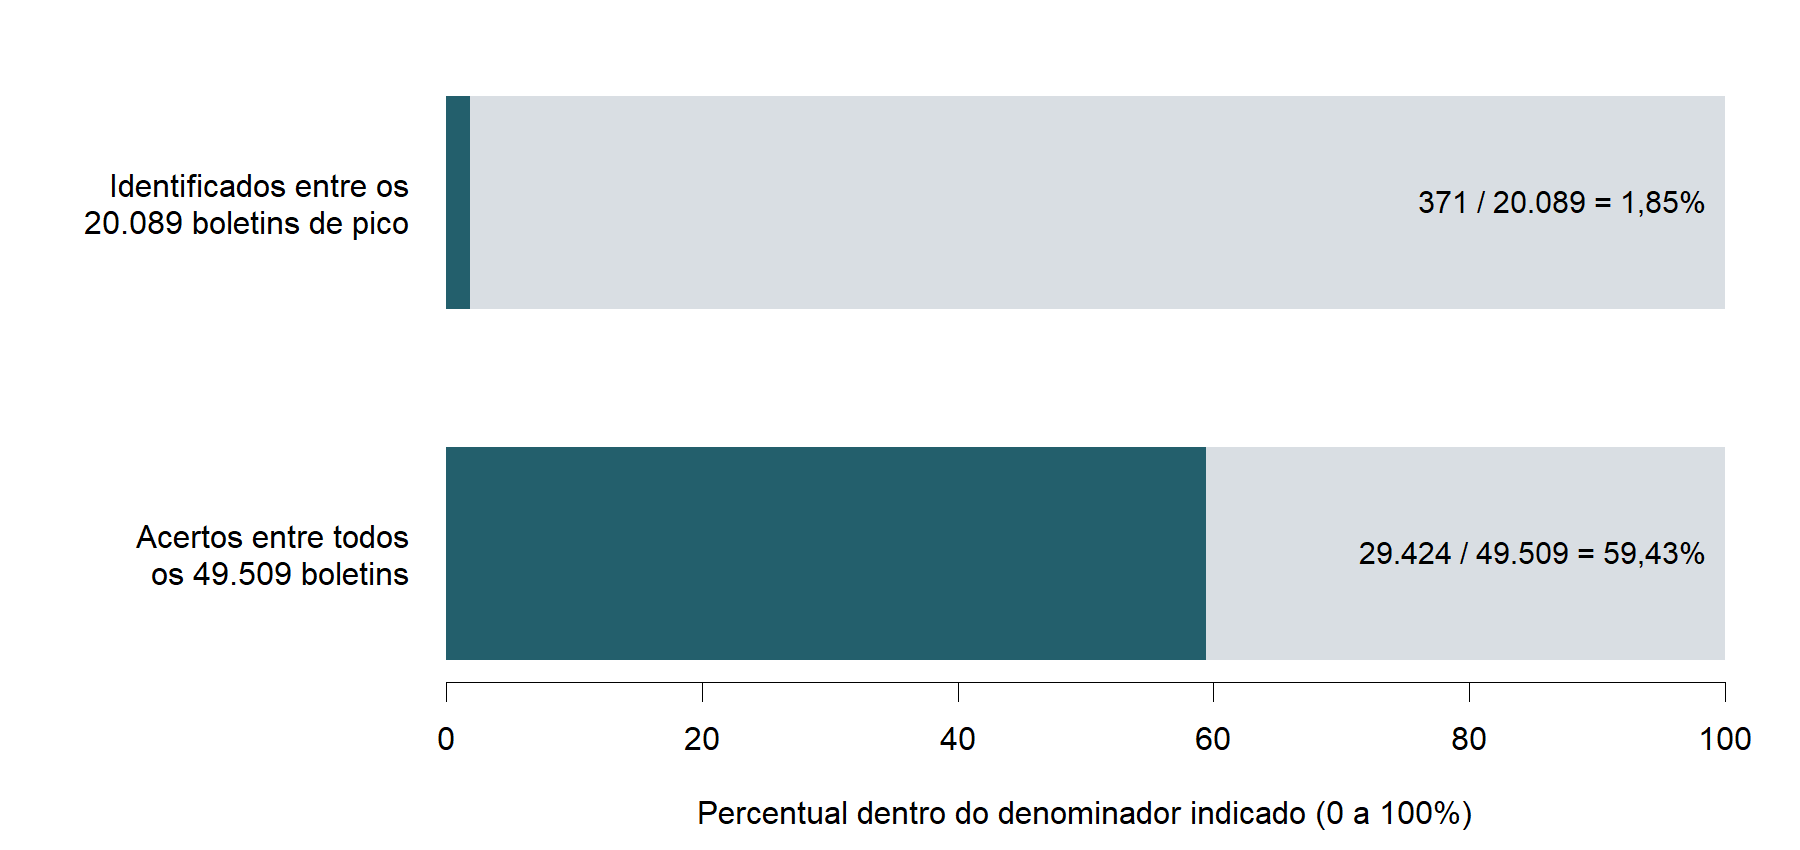
\includegraphics[width=0.68\linewidth]{figuras/acuracia-e-sensibilidade.png}
  \fonte{Elaborada pelos autores a partir dos dados do Infosiga-SP \parencite{infosiga2026}.}
\end{figure}

\begin{figure}[htbp]
  \centering
  \SingleSpacing
  \caption{Curva ROC e calibração por faixas das probabilidades previstas no teste de 2026}
  \label{fig:roc}
  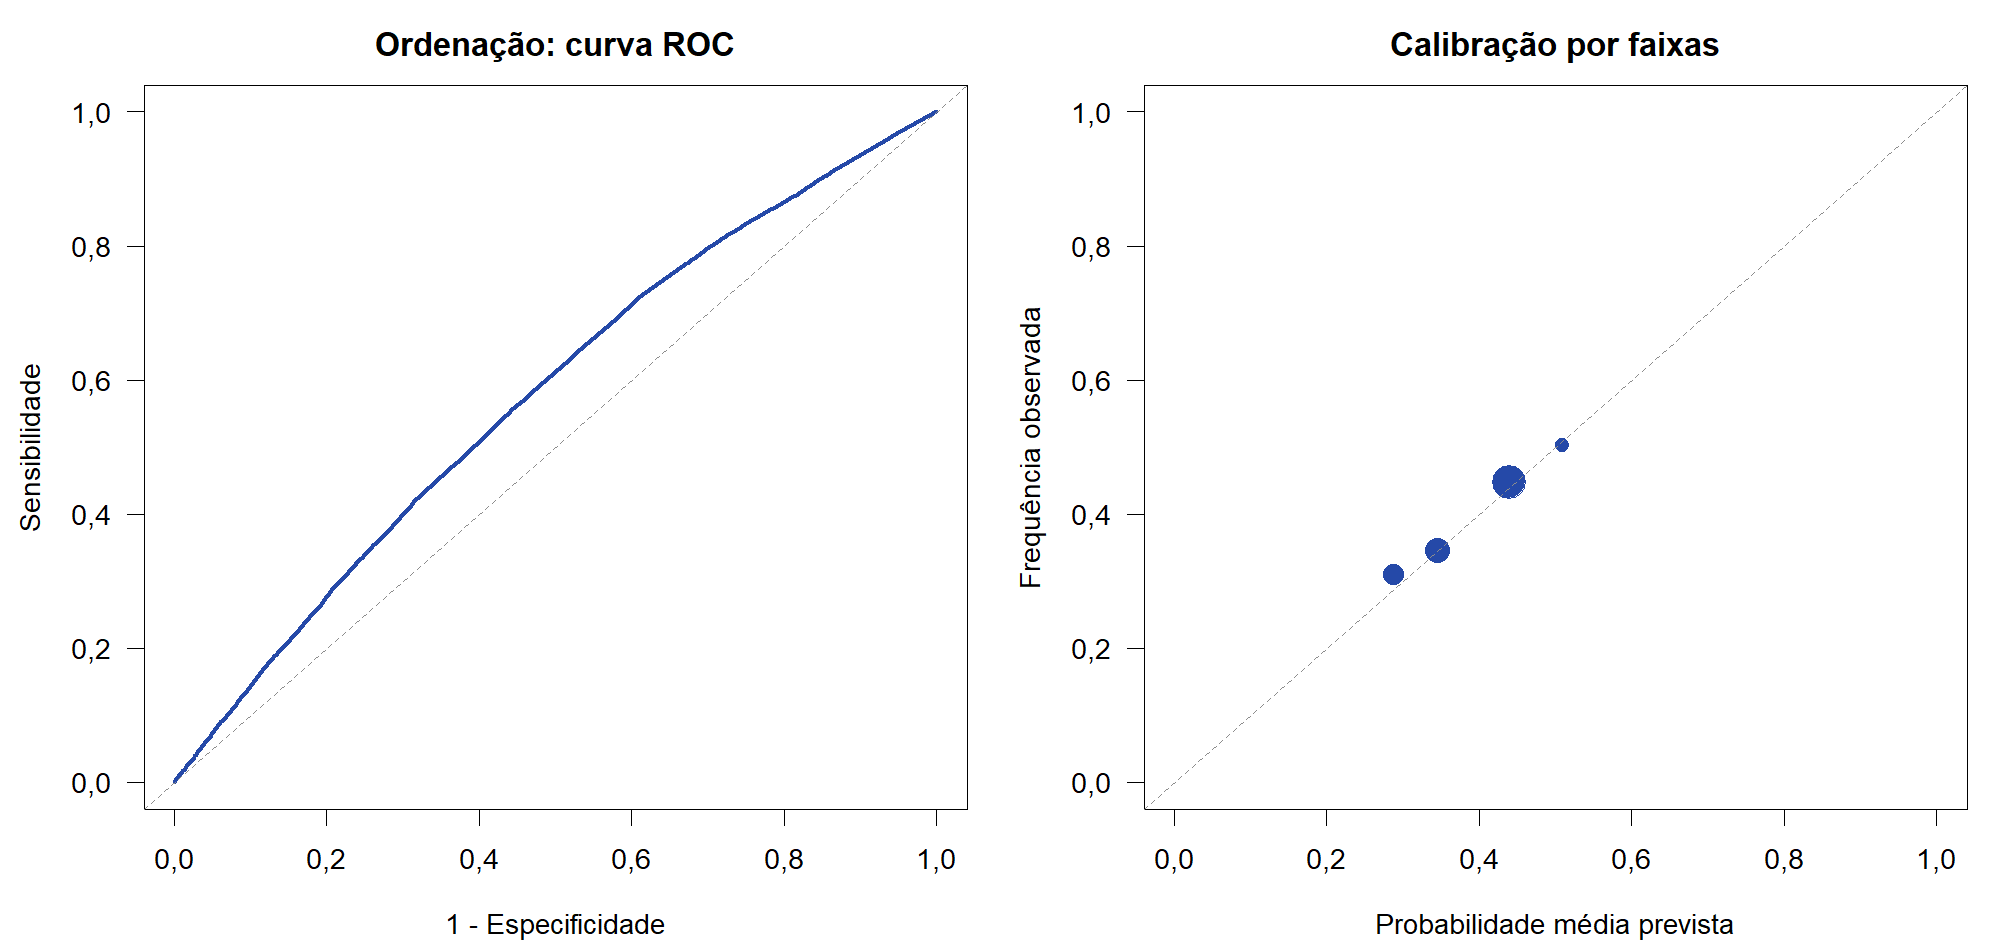
\includegraphics[width=0.76\linewidth]{figuras/roc-calibracao.png}
  \fonte{Elaborada pelos autores a partir dos dados do Infosiga-SP \parencite{infosiga2026}. À direita, o tamanho dos círculos cresce com $n$.}
\end{figure}

A Figura~\ref{fig:roc} exibe a curva ROC e o gráfico de calibração por faixas: as quatro faixas entre $(0{,}2; 0{,}6]$ acompanham visualmente a diagonal, embora o teste agrupado por data rejeite calibração perfeita (intercepto $= \text{0,0221}$; inclinação $= \text{0,9756}$; $\chi^2(2) = \text{10,7884}$; $p = \text{0,0045}$) pelo leve deslocamento de prevalência de $39{,}97\%$ para $40{,}58\%$. Nos testes conjuntos de Wald HC1 sobre os 365 dias de 2025 com ajuste de \textcite{holm1979}, confirmam-se associações fortes de \texttt{dia} ($\chi^2(6) = 952{,}355$; $p_{\mathrm{Holm}} < 0{,}0001$) e \texttt{regiao} ($\chi^2(15) = 284{,}839$; $p_{\mathrm{Holm}} < 0{,}0001$), enquanto \texttt{via} fica na fronteira de 5\% tanto no teste LR sob independência ($\chi^2(1) = \text{3,792}$; $p = \text{0,0515}$) quanto no Wald agrupado ($\chi^2(1) = \text{3,618}$; $p_{\mathrm{Holm}} = \text{0,0572}$). O bootstrap circular em blocos de sete dias (condicional ao ajuste de 2025) estimou contraste de Brier de 0,003972 (IC~95\% 0,003421--0,004472), e a AUC mensal manteve-se uniforme entre 0,5599 (fev.) e 0,5832 (mai.).

% ==============================================================================
\section{Discussão}
% ==============================================================================

A coexistência de $59{,}43\%$ de acurácia com $1{,}85\%$ de sensibilidade não decorre de desequilíbrio severo ($40{,}58\%$ dos registros de teste pertencem ao pico), mas da baixa variância explicada pelas três preditoras contextuais aditivas: $98{,}51\%$ das probabilidades previstas concentram-se abaixo de $\tau = 0{,}5$ (faixa de $0{,}2834$ a $0{,}5178$; mediana $0{,}4131$). Na escala contínua da probabilidade, o RMSE --- equivalente a $\sqrt{\mathrm{Brier}}$ em desfecho binário --- caiu apenas de 0,491077 para 0,487015 (diferença de 0,004061), confirmando ganho probabilístico modesto e ordenando os modelos de forma idêntica ao Brier ($\Delta = 0{,}003972$). Como alertam \textcite{bruce2019} e \textcite{lones2024}, relatar apenas acurácia global ou ajustar novo limiar sobre 2026 ocultaria o descarte de $19.718$ casos positivos.

Embora testes agrupados confirmem que \texttt{dia} e \texttt{regiao} possuem associação condicional estatisticamente detectável, significância em grandes amostras ($n > 100.000$) não equivale a poder preditivo operacional \parencite{james2021}. O modelo aditivo atribui probabilidade idêntica a boletins com a mesma combinação $(\text{via}, \text{dia}, \text{regiao})$, ignorando possíveis interações sazonais ou regionais. Portanto, com ganho líquido de apenas quatro acertos em $\tau = 0{,}5$, o ajuste é insuficiente como classificador operacional, mantendo utilidade exclusivamente descritiva para analisar como contexto viário, calendário e região se associam aos boletins registrados.

Quatro limitações restringem esse alcance: (1) ausência de denominadores de fluxo veicular para estimar risco relativo ou causalidade \parencite{who2010}; (2) perda seletiva de boletins fatais nas exclusões (656 de 658); (3) janelas estaduais uniformes sem validação local por congestionamento; e (4) caráter retrospectivo da avaliação sobre 2026 já explorado previamente na disciplina \parencite{lones2024,kapoor2024}.

% ==============================================================================
\section{Conclusão}
% ==============================================================================

Este estudo avaliou a associação entre características contextuais básicas (tipo de via, dia da semana e região administrativa) e a ocorrência de sinistros de trânsito em horários de pico no Estado de São Paulo, utilizando 151.175 boletins policiais válidos do Infosiga-SP em uma regressão logística treinada em 2025 ($n = 101.666$) e testada no primeiro semestre de 2026 ($n = 49.509$).

Embora os dias úteis apresentem associação estatisticamente detectável com os registros nos horários de pico em relação ao domingo, os resultados demonstram que a significância estatística em grandes amostras não se traduz em poder preditivo operacional. No teste temporal sob limiar de 0,5, o modelo obteve 59,43\% de acurácia --- apenas quatro acertos acima da referência constante de 59,42\% --- e apenas 1,85\% de sensibilidade (371 de 20.089 casos identificados), acompanhados por um ganho probabilístico modesto (AUC de 0,5757 e escore de Brier de 0,237184 ante 0,241157).

Por fim, a ausência de dados de fluxo veicular impede estimar risco por veículo em circulação, e a perda concentrada de registros fatais nas exclusões (656 de 658) recomenda cautela na generalização dos achados. Assim, ações de fiscalização e gestão viária não devem se apoiar exclusivamente em um corte binário de 0,5 baseado apenas nessas variáveis, cabendo a estudos futuros incorporar métricas de exposição de tráfego e validações prospectivas em novos períodos.

% ==============================================================================
% ELEMENTOS PÓS-TEXTUAIS (ABNT NBR 6022:2018 e NBR 6023:2018)
% ==============================================================================
\postextual
\printbibliography[title={REFERÊNCIAS}]

\clearpage
\appendix
\begin{SingleSpace}
\section*{APÊNDICE A -- RELATÓRIO DO AJUSTE NO R}
\addcontentsline{toc}{section}{APÊNDICE A -- RELATÓRIO DO AJUSTE NO R}
\noindent{\footnotesize Saída integral de \texttt{summary(modelo)} no treino de 2025 ($n = 101.666$), com erros-padrão convencionais de máxima verossimilhança; os erros-padrão robustos HC1 agrupados por data constam na Tabela~\ref{tab:coefs}.}
\begin{flushleft}\fontsize{7.2}{8.4}\selectfont
\begin{knitrout}
\definecolor{shadecolor}{rgb}{0.969, 0.969, 0.969}\color{fgcolor}\begin{kframe}
\begin{verbatim}

Call:
glm(formula = pico ~ via + dia + regiao, family = binomial(link = "logit"),
    data = treino)

Coefficients:
                                 Estimate Std. Error z value Pr(>|z|)
(Intercept)                      -0.64419    0.04884  -13.19  < 2e-16 ***
viaVIAS URBANAS                  -0.03424    0.01757   -1.95  0.05133 .
diaQuarta-feira                   0.60903    0.02547   23.91  < 2e-16 ***
diaQuinta-feira                   0.56485    0.02575   21.94  < 2e-16 ***
diaSábado                         0.02297    0.02605    0.88  0.37803
diaSegunda-feira                  0.53500    0.02565   20.86  < 2e-16 ***
diaSexta-feira                    0.39267    0.02508   15.66  < 2e-16 ***
diaTerça-feira                    0.61663    0.02563   24.06  < 2e-16 ***
regiaoBAIXADA SANTISTA           -0.18820    0.05155   -3.65  0.00026 ***
regiaoBARRETOS                   -0.22888    0.08232   -2.78  0.00543 **
regiaoBAURU                      -0.06037    0.05972   -1.01  0.31207
regiaoCAMPINAS                   -0.06551    0.04582   -1.43  0.15284
regiaoCENTRAL                     0.01027    0.06107    0.17  0.86646
regiaoFRANCA                      0.00819    0.06385    0.13  0.89794
regiaoITAPEVA                     0.03802    0.07724    0.49  0.62252
regiaoMARÍLIA                    -0.03449    0.05641   -0.61  0.54092
regiaoMETROPOLITANA DE SÃO PAULO -0.24910    0.04368   -5.70  1.2e-08 ***
regiaoPRESIDENTE PRUDENTE         0.05557    0.05546    1.00  0.31639
regiaoREGISTRO                   -0.22553    0.08346   -2.70  0.00689 **
regiaoRIBEIRÃO PRETO             -0.04860    0.05528   -0.88  0.37929
regiaoSÃO JOSÉ DO RIO PRETO       0.09872    0.05015    1.97  0.04903 *
regiaoSÃO JOSÉ DOS CAMPOS        -0.10640    0.05003   -2.13  0.03345 *
regiaoSOROCABA                   -0.12147    0.04956   -2.45  0.01424 *
---
Signif. codes:  0 '***' 0.001 '**' 0.01 '*' 0.05 '.' 0.1 ' ' 1

(Dispersion parameter for binomial family taken to be 1)

    Null deviance: 136819  on 101665  degrees of freedom
Residual deviance: 135094  on 101643  degrees of freedom
AIC: 135140

Number of Fisher Scoring iterations: 4
\end{verbatim}
\end{kframe}
\end{knitrout}
\end{flushleft}
\end{SingleSpace}

\end{document}
